%Copyright 2014 Jean-Philippe Eisenbarth
%This program is free software: you can 
%redistribute it and/or modify it under the terms of the GNU General Public 
%License as published by the Free Software Foundation, either version 3 of the 
%License, or (at your option) any later version.
%This program is distributed in the hope that it will be useful,but WITHOUT ANY 
%WARRANTY; without even the implied warranty of MERCHANTABILITY or FITNESS FOR A 
%PARTICULAR PURPOSE. See the GNU General Public License for more details.
%You should have received a copy of the GNU General Public License along with 
%this program.  If not, see <http://www.gnu.org/licenses/>.

%Based on the code of Yiannis Lazarides
%http://tex.stackexchange.com/questions/42602/software-requirements-specification-with-latex
%http://tex.stackexchange.com/users/963/yiannis-lazarides
%Also based on the template of Karl E. Wiegers
%http://www.se.rit.edu/~emad/teaching/slides/srs_template_sep14.pdf
%http://karlwiegers.com
\documentclass{scrreprt}
\usepackage{listings}
\usepackage{underscore}
\usepackage[bookmarks=true]{hyperref}
\usepackage[utf8]{inputenc}
\usepackage[english]{babel}
\usepackage{xcolor,colortbl}
\usepackage{makecell}
\usepackage{graphicx}
\hypersetup{
	bookmarks=false,    % show bookmarks bar?
	pdftitle={High-leve Design Document},    % title
	pdfauthor={Mohammad Arastu, Raphael Arzberger, Martin Fuhrmann},                     % author
	pdfsubject={TeX and LaTeX},                        % subject of the document
	pdfkeywords={TeX, LaTeX, graphics, images}, % list of keywords
	colorlinks=true,       % false: boxed links; true: colored links
	linkcolor=blue,       % color of internal links
	citecolor=black,       % color of links to bibliography
	filecolor=black,        % color of file links
	urlcolor=purple,        % color of external links
	linktoc=page            % only page is linked
}%
\newcolumntype{L}[1]{>{\raggedright\let\newline\\\arraybackslash\hspace{0pt}}m{#1}}
\newcolumntype{C}[1]{>{\centering\let\newline\\\arraybackslash\hspace{0pt}}m{#1}}
\newcolumntype{R}[1]{>{\raggedleft\let\newline\\\arraybackslash\hspace{0pt}}m{#1}}
\def\myversion{1.0}
\definecolor{LightCyan}{rgb}{0.88,1,1}
\date{}
%\title
\usepackage{hyperref}
\begin{document}
	
	\begin{flushright}
		\rule{16cm}{5pt}\vskip1cm
		\begin{bfseries}
			\Huge{High Level Design Document}\\
			\vspace{1.9cm}
			for\\
			\vspace{1.9cm}
			Timetable Planner\\
			\vspace{1.9cm}
			\LARGE{Version \myversion}\\
			\vspace{1.9cm}
			Prepared by \\ {\small Mohamad Arastu, Raphael Arzberger, Martin Fuhrmann}
			\vspace{1.9cm} \\
			\today\\
		\end{bfseries}
	\end{flushright}
	
	\tableofcontents
	
	
	\chapter*{Revision History}
	
	\begin{center}
		\begin{tabular}{|c|c|c|c|}
			\hline
			Date & Reason For Changes & Responsible Person & Version\\
			\hline
			06.12.2022 & project start & Mohammad Arastu, & \\&&Raphael Arzberger, & \\&&Martin Fuhrmann & 0.1\\
			\hline
			11.12.2022 & added diagrams and description & Mohammad Arastu, & \\&&Raphael Arzberger, & \\&&Martin Fuhrmann & 1.0\\
			\hline
		\end{tabular}
	\end{center}
	
	\chapter{Introduction}
	
	\section{Purpose}
	Currently the timetable of the course of study for 'Computer Science and Digital Communications' is still being set up manually without any tool support.\\\\
	Consider the following:\\
	Every student is assigned a group and each of those groups has an individual timetable that needs to be consistent in itself. Some lecture courses should be finished earlier	within a semester than others, meaning a time window has to be considered for every course when setting up the timetable for a specific year group. Moreover, there might a predefined sequence of lectures and exercises for a course, some lecturers might only be available on certain days of the week, different courses taking	place on the same day should all be either online or on-site, students might want that exams are well spread over time to balance work load, ... etc.\\\\
	Having a look at the vast number of constraints that have to be considered in setting up the timetable one can easily imagine that this is a time-consuming and tedious task when done without any tool support. Therefore, a software support should be developed that allows an efficient way to set up consistent timetables for each group


	
	\section{System Overview}
	The system consists of different components: User input, Data validation, Timetable creation, Timetable validation, Timetable export
	\chapter{Component Overview}
	User input: User provides the program with needed data\\
	Data validation: The program validates the given data\\
	Timetable creation: The algorithm creates a timetable\\
	Timetable validation: The timetable is validated\\
	TimeTable export: Exporting the timetable in a human readable way\\
	
	\chapter{Detailed Design}
	\section{Architecture}
	\section{UML Diagrams}
	\subsection{Class Diagram}
	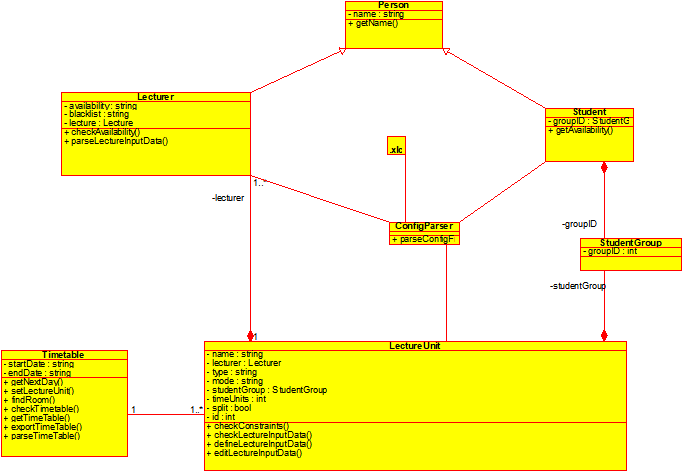
\includegraphics{class diagram}
	\subsection{Activity Diagram}
	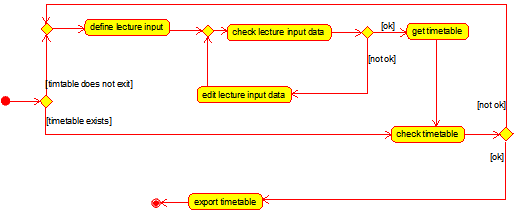
\includegraphics{activity diagram}
	\subsection{Sequence Diagram}
	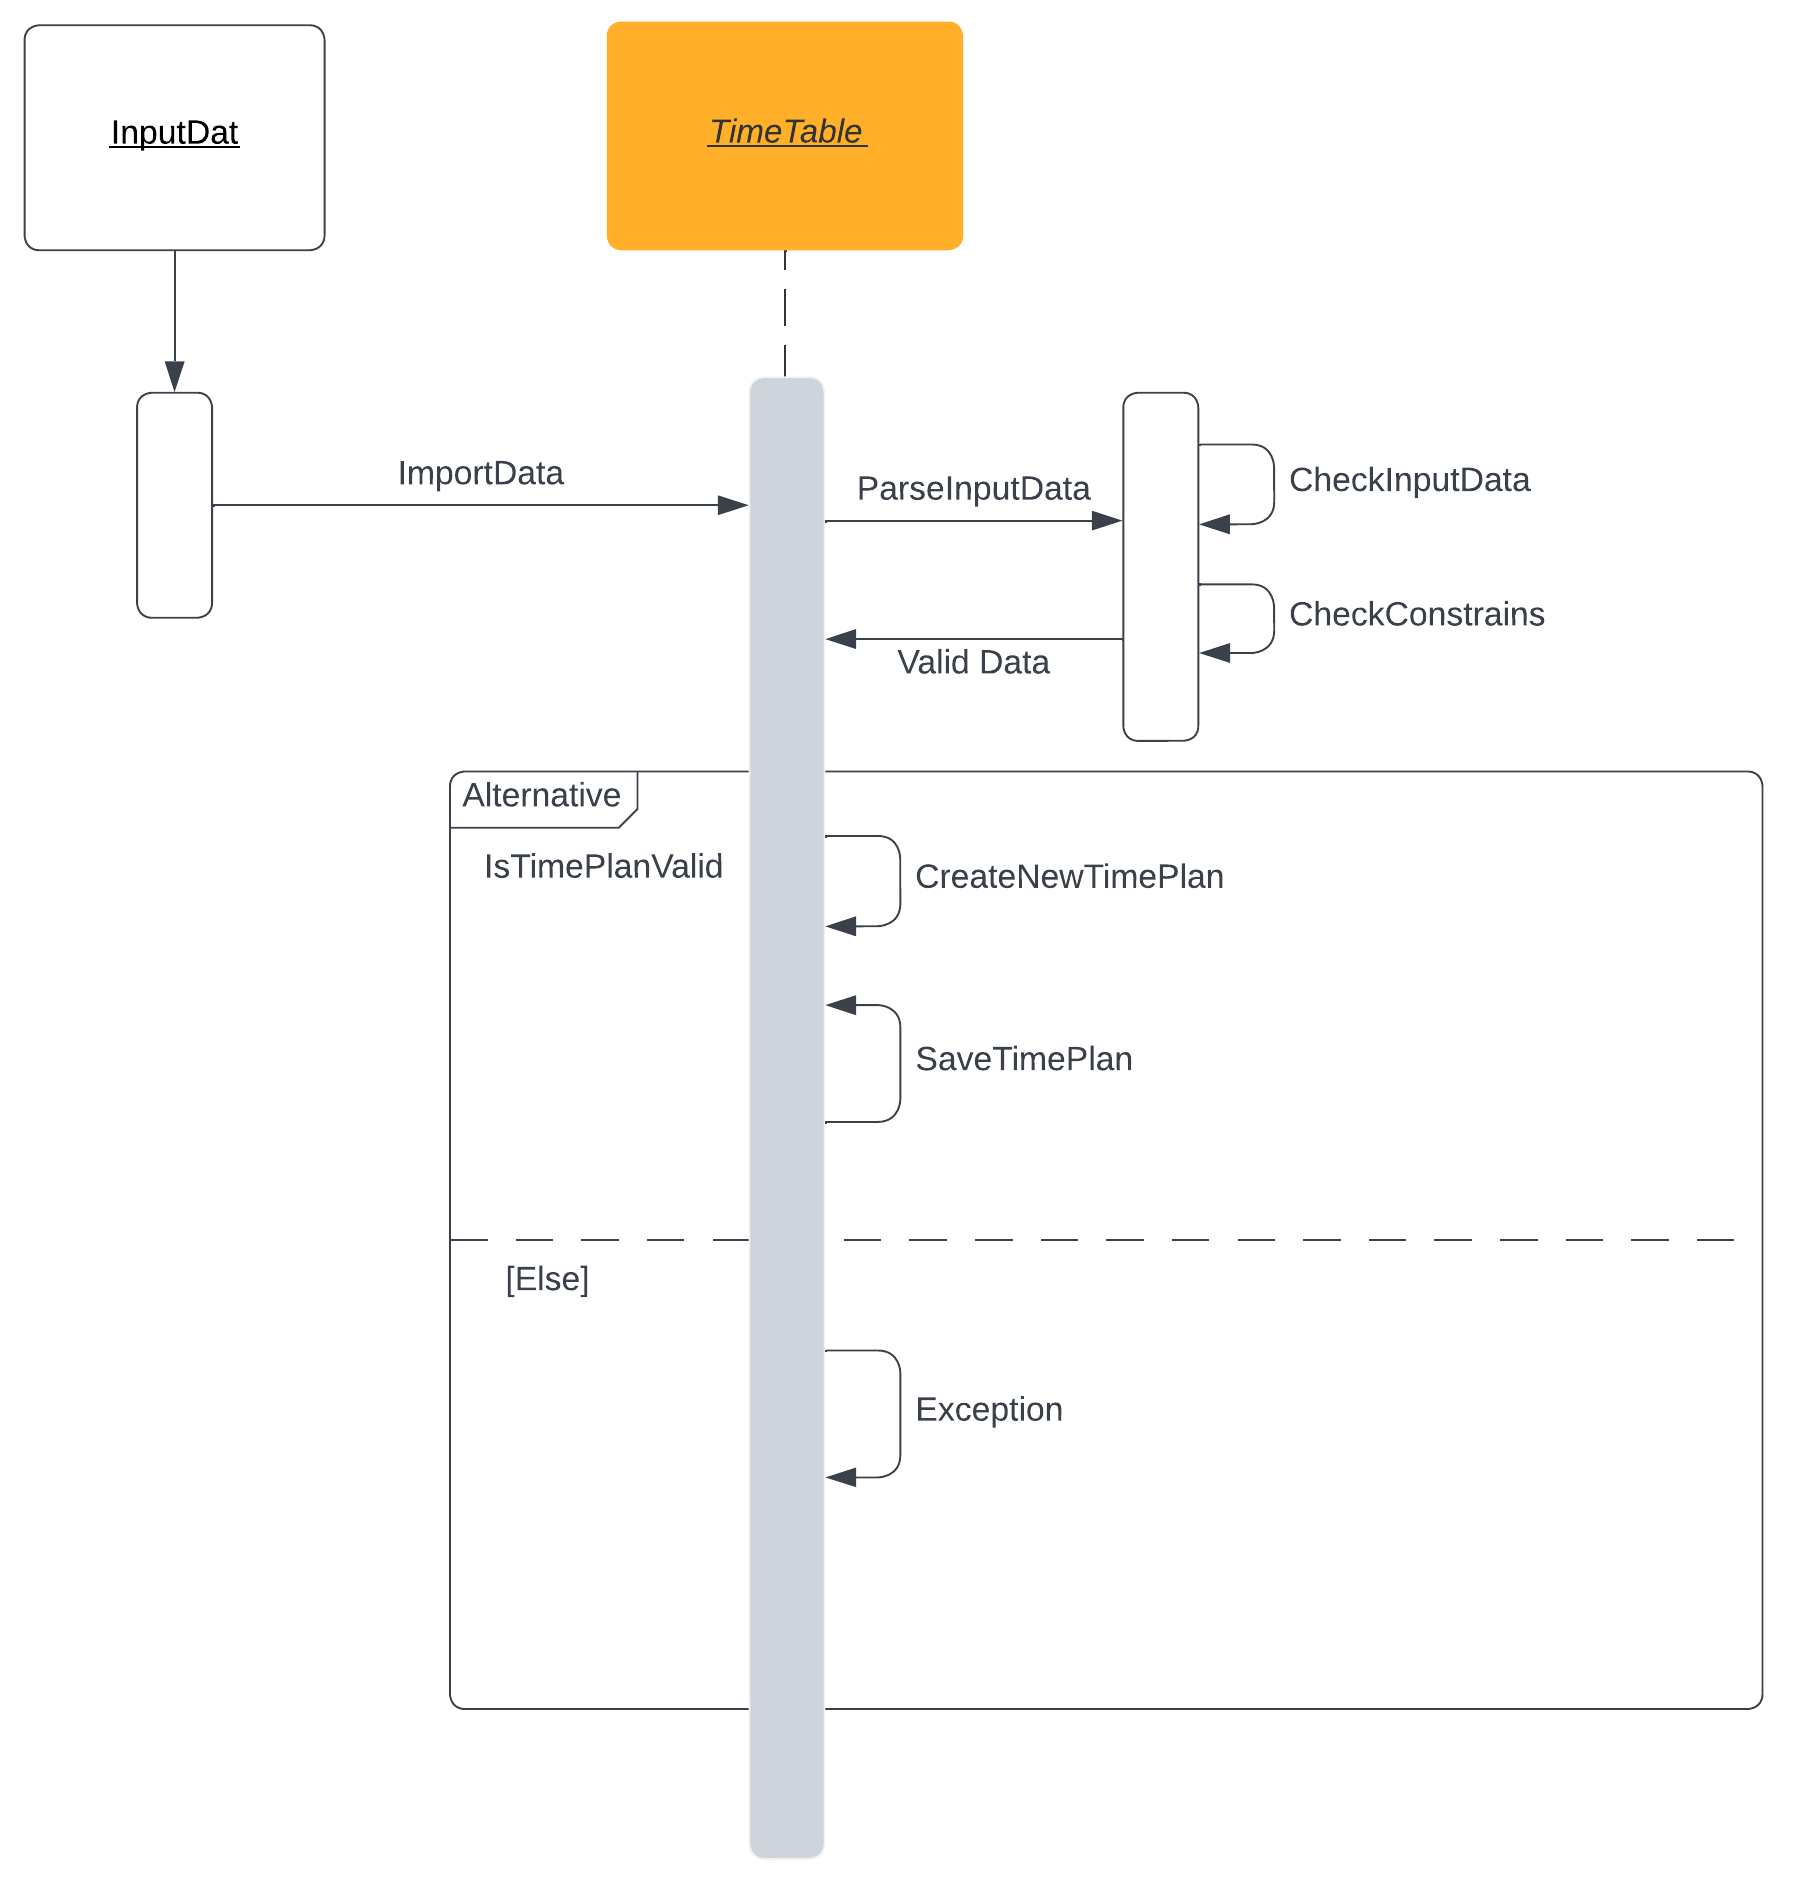
\includegraphics{Sequence diagram NO DB}
	
	
\end{document}
